\documentclass{notices}
\usepackage{graphicx}
\usepackage{subcaption}
\usepackage{adjustbox}
\usepackage{multicol}
\usepackage{adjmulticol}
\usepackage{graphicx}
\usepackage{caption}
\usepackage[bbgreekl]{mathbbol}
\usepackage{tkz-graph}
\usepackage{subcaption}
\usepackage{tikz}
\usetikzlibrary{arrows.meta, decorations.pathreplacing, arrows,shapes,positioning}
\usepackage{float}
\usepackage{sectsty}
\usepackage{amsrefs}
\usepackage{titlesec,amsthm}
\setlength{\columnsep}{0.33in}
\usepackage[margin=0.95in]{geometry}



\theoremstyle{definition}\newtheorem{problem}{Problem}

\sectionfont{\fontsize{12}{15}\selectfont}

%
% --- inline annotations
%
\newcommand{\red}[1]{{\color{red}#1}}
\newcommand{\todo}[1]{{\color{red}#1}}
\newcommand{\TODO}[1]{\textbf{\color{red}[TODO: #1]}}
% --- disable by uncommenting  
% \renewcommand{\TODO}[1]{}
% \renewcommand{\todo}[1]{#1}



\newcommand{\VLM}{LVLM\xspace} 
\newcommand{\ours}{PeKit\xspace}
\newcommand{\yollava}{Yo’LLaVA\xspace}

\newcommand{\thisismy}{This-Is-My-Img\xspace}
\newcommand{\myparagraph}[1]{\noindent\textbf{#1}}
\newcommand{\vdoro}[1]{{\color[rgb]{0.4, 0.18, 0.78} {[V] #1}}}
% --- disable by uncommenting  
% \renewcommand{\TODO}[1]{}
% \renewcommand{\todo}[1]{#1}
\usepackage{slashbox}
% Vectors
\newcommand{\bB}{\mathcal{B}}
\newcommand{\bw}{\mathbf{w}}
\newcommand{\bs}{\mathbf{s}}
\newcommand{\bo}{\mathbf{o}}
\newcommand{\bn}{\mathbf{n}}
\newcommand{\bc}{\mathbf{c}}
\newcommand{\bp}{\mathbf{p}}
\newcommand{\bS}{\mathbf{S}}
\newcommand{\bk}{\mathbf{k}}
\newcommand{\bmu}{\boldsymbol{\mu}}
\newcommand{\bx}{\mathbf{x}}
\newcommand{\bg}{\mathbf{g}}
\newcommand{\be}{\mathbf{e}}
\newcommand{\bX}{\mathbf{X}}
\newcommand{\by}{\mathbf{y}}
\newcommand{\bv}{\mathbf{v}}
\newcommand{\bz}{\mathbf{z}}
\newcommand{\bq}{\mathbf{q}}
\newcommand{\bff}{\mathbf{f}}
\newcommand{\bu}{\mathbf{u}}
\newcommand{\bh}{\mathbf{h}}
\newcommand{\bb}{\mathbf{b}}

\newcommand{\rone}{\textcolor{green}{R1}}
\newcommand{\rtwo}{\textcolor{orange}{R2}}
\newcommand{\rthree}{\textcolor{red}{R3}}
\usepackage{amsmath}
%\usepackage{arydshln}
\DeclareMathOperator{\similarity}{sim}
\DeclareMathOperator{\AvgPool}{AvgPool}

\newcommand{\argmax}{\mathop{\mathrm{argmax}}}     


\allowdisplaybreaks

\titlespacing*{\section}
{0pt}{1.5ex plus 1ex minus .2ex}{0.5ex plus .2ex}

\def\eproof{\hfill \hbox{\hskip3pt\vrule width4pt height8pt depth1.5pt}}

\def\eproofwhite{\hfill $\square$}



\title{
Eigenvalues in microeconomics
}


\author{
  Benjamin Golub
  \affil{
    The  author is a professor of economics and computer science at Northwestern. His email address is bgolub@northwestern.edu.
    }
}


\begin{document}

\maketitle

Square matrices often appear in formal models of social and economic behavior, especially models involving networks. Such models are used to study subjects ranging from opinion dynamics to pollution-mitigation negotiations to the regulation of large marketplace platforms such as Amazon.  Typically, the square matrices that arise represent a suitable notion of nodes' ``marginal influence'' on one another. Spectral theory offers powerful tools for studying such matrices, and so underlies many key insights about these models. The Perron--Frobenius Theorem on nonnegative eigenvectors has played an especially prominent role in network applications. This essay uses these unifying mathematical threads to offer an accessible tour of several important ideas in social science, assuming minimal non-mathematical background knowledge. Though the tour is necessarily brief, references cited throughout supply more context.



\section*{Central Notions}

We start with a few standard definitions from the theory of nonnegative matrices that will play a recurring role. The applications that follow will provide motivation and intuition.

We will associate an $n$-by-$n$ matrix $M$ with a weighted digraph on the nodes \([n]=\{1,2,\ldots,n\}\), whose edges are all ordered pairs \((i,j)\) with \(M_{ij} > 0\). The matrix is called irreducible if this digraph is strongly connected. 

The \emph{spectral radius} of a matrix $M$, denoted by $\rho(M)$, is defined to be the maximum modulus of its eigenvalues.

\begin{thmNoNum}[Perron--Frobenius]
Let \(n \ge 2\), and let \(M\) be an \(n\times n\) nonnegative, irreducible matrix. Then:
\begin{enumerate}
    \item \(M\) has a positive real eigenvalue \(\lambda\) equal to its spectral radius \(\rho(M)\).
    \item There are uniquely determined vectors \(c, r \in \mathbb{R}^n_{>0}\) such that \(c^\top M = \lambda\,c^\top\) and \(Mr = \lambda\,r\).
    \item Any nonnegative left (resp., right) eigenvector of \(M\) with any positive eigenvalue is a scalar multiple of \(c^\top\) (resp. \(r\)).
\end{enumerate}
\end{thmNoNum}

In network theory, the entries of $c^\top$ are called agents' (left-hand) \emph{eigenvector centralities} in the $M$ digraph. The system of equations \begin{equation} \label{eq:centrality} \lambda c_i=\sum_j c_j M_{ji}  \text{ for each $i$},\end{equation} defining the eigenvector $c^\top$ says that node $i$'s centrality is a weighted sum of others' centralities, with $c_j$ contributing in proportion to the weight of the link from $j$ to $i$ in the digraph.

Well before the models of behavior we are about to discuss were proposed, sociologists were interested in centralities $c_i$ satisfying \cref{eq:centrality} as a standalone measure of the importance, connectedness, or status of nodes in a network. The idea that ``the cool kids are the ones who receive respect from the cool kids'' is made plausible for many of us by memories of high school, and the centrality equation captures this fixed-point property in a linear form. Note that nothing anchors eigenvector centralities to any external source of node values;  \cref{eq:centrality} contains no constant terms. It might therefore seem possible to consistently assign centralities to satisfy the equation in many different ways. Remarkably, however, the Perron--Frobenius Theorem guarantees that relative eigenvector centralities are uniquely determined within a strongly connected component. We now turn to some implications of this fundamental result.



\section*{Social Influence}

An adage that rings true to me is, ``You are the average of the five people you spend the most time with.'' A simple yet surprisingly illuminating model of social learning---named for the statistician Morris DeGroot \cite{degroot1974reaching}---takes this idea seriously.

Consider a set of $n \geq 2$ agents (the word we will use for people, though they could also be, say, robots), each with an evolving \emph{opinion} of some quantity of interest. The opinion of agent $i$ is an element $x_i \in V$, where $V$ is a convex subset of a finite-dimensional vector space equipped with an inner product. To take some examples, we can think of the opinion $x_i$ as a number describing how good Taylor Swift's music is on a scale of 0 to 100; a probability distribution over some set $\Omega$ describing beliefs about the future of climate change (where $\Omega$ describes various dimensions of the observable world);  or a vector representation of how agent $i$ pronounces a particular word, defined via an embedding from modern machine learning models. In the DeGroot model, in each period, agents update their opinions by taking weighted averages of opinions from the previous period, possibly including their own. The vector\footnote{Vectors are column vectors by default.} of opinions at time $t$, denoted by $x(t) \in V^n$, evolves according to:
$$ x(t+1) = Mx(t) \quad \text{for $t=0,1,2,\ldots$}$$ The data of this process are the $n$-by-$n$ row-stochastic matrix $M$ and the vector of initial opinions $x(0)$, with $M_{ij} \geq 0$ representing the weight agent $i$ places on agent $j$'s most recent opinion. One interpretation is that \(M_{ij} > 0\) only if \(i\) has access to \(j\)'s opinion (e.g., because \(i\) knows \(j\) personally or follows \(j\) on social media), and the magnitude of \(M_{ij}\) reflects how much \(i\) is influenced by \(j\).  We will typically dispense with the generality of an arbitrary $V$ and focus on the case $V=\mathbb{R}$ from now on.



The dynamics of the process are very simple: $x(t) = M^t x(0)$. Can agents in this model disagree forever? Under some natural conditions, the answer is no. The conditions concern the digraph associated to $M$. Recall that this digraph is called \emph{aperiodic} if the greatest common divisor of the lengths of all its directed cycles is $1$. Let $\Delta_n$ denote the set of probability distributions on $[n]$, viewed as row vectors.

\begin{fact} \label{fact:degroot_convergence} If the digraph of $M$ is strongly connected and aperiodic, opinions converge to a consensus, meaning that $\lim_{t \to \infty} x(t) = a \mathbf{1}$ for some $a \in V$, where $\mathbf{1}$ is the vector of ones. In this case, the consensus opinion $a$ is determined by the unique left eigenvector $c^\top \in \Delta_n$ of $M$  corresponding to the eigenvalue 1:
$$ a = c^\top x(0). $$
\end{fact}

The existence and uniqueness of the eigenvector $c$ follow from the Perron--Frobenius theorem.\footnote{Since the strictly positive vector $\bm{1}$ is a right eigenvector of $M$ with eigenvalue $1$, the theorem gives that $1$ is a largest eigenvalue of $M$ and comes with a left eigenvector $c^\top$.} 

Our characterization of consensus follows from the fact, familiar from the Markov chain perspective, that $\lim_{t \to \infty} M^t = \mathbf{1}  c^\top$---see \cite[Ch. 8]{meyer-book} for an excellent treatment. Indeed, $c^\top$ is simply the stationary distribution of the Markov chain associated with $M$. It is a fun exercise to establish that $x(t)$ converges to \emph{some} $a \in V$ by working directly with the DeGroot process $x(t) = M^t x(0)$, without appealing to any Markov chain results.\footnote{Nevertheless, the argument is likely to need the following elementary number-theoretic: $A$ is primitive (meaning that there is some such that $A^t$ has no entries equal to zero) if and only if its associated digraph is strongly connected and aperiodic.} The idea is that as long as disagreement remains in a strongly connected network, some agents must moderate their opinions in some bounded number of steps. This gives an alternative proof of the existence of  $\lim_{t\to \infty} M^t$.

Coming back to the substance of the model, the entries of $c$ can be interpreted as measures of agents' social influence, with $c_i$ representing the weight of agent $i$'s initial opinion in the long-run consensus. So while the local updating dynamics prescribe that an agent's opinion is the average of the ``five'' opinions in its neighborhood,  the process ultimately leads a strongly connected network to share a consensus opinion that blends all initial opinions---with particular weights.

The weights satisfy \cref{eq:centrality}. In the DeGroot model, it is natural that the influences are eigenvector centralities: influence comes from being listened to, and is increasing in the listeners' influences. However, one need not have many  connections to be highly central: some weight $M_{ij}$ from high-centrality nodes is enough. Note also that just as agents' \emph{opinions} in the DeGroot model are the averages of recent neighborhood opinions by assumption, agents' \emph{influences} end up having a related property: an agent is influential when that agent has influential in-neighbors. 


The behavior of these centralities in large graphs is interesting both mathematically and in applications. \cite{GolubJackson2010} considered a sequence $(M(n))_{n=1}^\infty$ of  irreducible stochastic matrices, with the matrix $M(n)$ having dimensions $n$-by-$n$, as a model of a large society. They asked whether the associated eigenvector centralities $c_i(n)$ uniformly converge to $0$. In this case $(M(n))_{n=1}^\infty$ is called \emph{wise}, motivated by the following story. Imagine the initial opinions $x_i(0)$ in network $n$ are drawn independently from distributions on $V$ with finite, positive variances and a common expectation $\mu$. If the consensus $a(n)$ converges in probability  to $\mu$, large communities enjoy the so-called wisdom of crowds: no individual's noisy opinion can obstruct convergence to the truth $\mu$. A weak law of large numbers implies that this happens if and only if $(M(n))_{n=1}^\infty$ is wise as we have defined it. 

We can identify a simple obstruction to wisdom. A sequence $(P(n))_{n=1}^\infty$  of nonempty subsets of nodes is \emph{prominent} if, for each $n$, there is a $t$ so that
$\sum_{i \in P(n)} (M(n)^t)_{ij} \geq \epsilon$ for all $j \notin P(n)$,
where $\epsilon > 0$ is fixed across $n$. Intuitively, such a sequence is one that collectively has significant influence on all other agents after some number of updating rounds.
\begin{prop}  The sequence $(M(n))_{n=1}^\infty$ is wise if and only if there is no prominent sequence where $|P(n)|$ is uniformly bounded. \end{prop}
Because of the quantification over $t$ in the definition of prominence, the result is interesting mainly for quickly ruling out wisdom. \cite{GolubJackson2010} give some interpretable sufficient conditions for wisdom, but sharp and interpretable conditions are not known.

Natural generalizations of the DeGroot dynamic open up connections to topics of current interest in mathematics and open questions about opinion dynamics. \cite{CCL} study a class of nonlinear operators $T : \mathbb{R}^n \to \mathbb{R}^n$ generalizing the linear action of Markov matrix $M$ in the DeGroot model. They call an operator \emph{robust} if it is entrywise monotone and satisfies $T(x+\gamma \bm{1})=T(x)+\gamma T(\bm{1})$ for every constant $\gamma \in \mathbb{R}$. A very nice convergence theory exists for such operators in general spaces, and is surveyed in \cite{CCL,lemmens2012nonlinear}. A natural question generalizing the study of the wisdom of crowds is how much $T^\infty$ can depend on any small set of entries. For example, suppose we take an undirected Erdos-Renyi graph on $[n]$ with some edge probability $p(n) \gg \log(n)$ as a model of a connected social network. Fix symmetric functions $\tau_d$ for every possible degree $d$ in the network, and for each agent $i$ of degree $d_i$, let $T_i(x) = \tau((x_j)_{j \in N(i)})$ where $(x_j)_{j \in N(i)}$ are the opinions in the set $N(i)$ of $i$'s neighbors. If $\tau$ is chosen so that $T$ is robust in the sense above and has uniformly bounded derivatives, it seems natural to conjecture that an analogue of wisdom should hold. The intuitive reason is symmetry: agents' roles are exchangeable, and there seems to be nothing favoring the emergence of globally prominent roles by accident. \cite{CCL} make remarkable progress toward this conjecture under technical  assumptions on the second-largest eigenvalue of a matrix reflecting the social network. However, under important models of social networks---sparse Erdos--Renyi models, stochastic block models, models with agents arranged on a lattice---these technical assumptions would not hold. Better understanding how generalizations of centrality statistics behave in large networks is a wide open and exciting problem.



\section*{A Richer Centrality}



Eigenvector centralities were defined based on the network alone, with no other determinants of status or prestige. But sometimes such determinants are present. Incorporating them leads to a notion of centrality that extends the eigenvector equation by adding an exogenous term. Specifically, given a positive \emph{decay parameter} $\delta  < 1/\rho(M)$ and a vector $z \in \mathbb{R}^n$  the vector of  $(\delta,z)$--\emph{Katz--Bonacich centralities} 
$k$ is defined \cite{Jackson2008} to satisfy
\begin{equation} \label{eq:kb} k^\top = \delta k^\top M  + z^\top. \end{equation}
We will see some economic applications that give foundations to this equation, but on its own terms, one can think of high school students having external sources of status (such as mathematical ability) and one's social status coming from a (linear) combination of this external level and the status derived from one's in-connections.


\begin{figure}[t]
\centering
\begin{subfigure}[b]{0.48\textwidth}
    \centering
    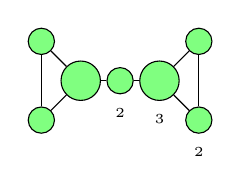
\begin{tikzpicture}[
        scale=0.5,
        node/.style={
            circle, 
            draw, 
            fill=green!50, 
            minimum size={2*((#1/3))*0.5*0.5cm},
            inner sep=0pt
        },
        label/.style={font=\tiny, align=center}
    ]
    \node[node=2] (1) at (3, 1) {};
    \node[node=2] (2) at (3, 3) {};
    \node[node=3] (3) at (2, 2) {};
    \node[node=2] (4) at (1, 2) {};
    \node[node=3] (5) at (0, 2) {};
    \node[node=2] (6) at (-1, 1) {};
    \node[node=2] (7) at (-1, 3) {};
    \node[label, below=0.05cm of 1] {2};
    \node[label, below=0.05cm of 3] {3};
    \node[label, below=0.05cm of 4] {2};
    \draw (1) -- (3); \draw (2) -- (3); \draw (3) -- (4);
    \draw (4) -- (5); \draw (5) -- (6); \draw (5) -- (7);
    \draw (1) -- (2); \draw (6) -- (7);
    \end{tikzpicture}
    \caption{}
    \label{fig:subfig-a}
\end{subfigure}
\hfill
\begin{subfigure}[b]{0.48\textwidth}
    \centering
    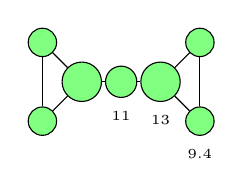
\begin{tikzpicture}[
        scale=0.5,
        node/.style={
            circle, 
            draw, 
            fill=green!50, 
            minimum size={2*((#1/6.8))*0.5*0.5cm},
            inner sep=0pt
        },
        label/.style={font=\tiny, align=center}
    ]
    \node[node=4.9] (1) at (3, 1) {};
    \node[node=4.9] (2) at (3, 3) {};
    \node[node=6.8] (3) at (2, 2) {};
    \node[node=5.4] (4) at (1, 2) {};
    \node[node=6.8] (5) at (0, 2) {};
    \node[node=4.9] (6) at (-1, 1) {};
    \node[node=4.9] (7) at (-1, 3) {};
    \node[label, below=0.05cm of 1] {9.4};
    \node[label, below=0.05cm of 3] {13};
    \node[label, below=0.05cm of 4] {11};
    \draw (1) -- (3); \draw (2) -- (3); \draw (3) -- (4);
    \draw (4) -- (5); \draw (5) -- (6); \draw (5) -- (7);
    \draw (1) -- (2); \draw (6) -- (7);
    \end{tikzpicture}
    \caption{}
    \label{fig:subfig-b}
\end{subfigure}

\bigskip

\begin{subfigure}{.48\textwidth}
    \centering
    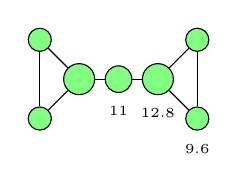
\begin{tikzpicture}[
        scale=0.5,
        node/.style={
            circle, 
            draw, 
            fill=green!50, 
            minimum size={2*((#1/80))*0.5*0.5cm},
            inner sep=0pt
        },
        label/.style={font=\tiny, align=center}
    ]
    \node[node=47] (1) at (3, 1) {};
    \node[node=47] (2) at (3, 3) {};
    \node[node=63] (3) at (2, 2) {};
    \node[node=54] (4) at (1, 2) {};
    \node[node=63] (5) at (0, 2) {};
    \node[node=47] (6) at (-1, 1) {};
    \node[node=47] (7) at (-1, 3) {};
    \node[label, below=0.05cm of 1] {9.6};
    \node[label, below=0.05cm of 3] {12.8};
    \node[label, below=0.05cm of 4] {11};
    \draw (1) -- (3); \draw (2) -- (3); \draw (3) -- (4);
    \draw (4) -- (5); \draw (5) -- (6); \draw (5) -- (7);
    \draw (1) -- (2); \draw (6) -- (7);
    \end{tikzpicture}
    \caption{}
    \label{fig:subfig-c}
\end{subfigure}
\caption{Nodes sized proportional to (a) degree centrality; (b) Bonacich centrality with $z=\bm{1}$ and $\delta=1/3$; (c) eigenvector centrality, which we see is similar since $\delta M$ has spectral radius not far from $1$.}
\label{fig:combined}
\end{figure}

The fact that $\rho(\delta M)<1$ allows us to use the Neumann series expansion $k^\top = z^\top \sum_{t=0}^\infty \delta^t M^t $, which shows that $i$'s Katz--Bonacich centrality is a sum of the weights of incoming walks (entries of $(M^)_{ij}$) weighted by $z_j$ (where those walks end). In particular, it is uniquely defined. Moreover, as $\delta \rho(M)$ approaches $1$ from below---the boundary at which the Neumann series diverges---the suitably rescaled Katz--Bonacich centrality $(1-\delta)k(\delta)$ converges\footnote{Proving this is a good exercise. A quick guide: reduce to the case where $\rho(M)=1$ and $z^\top \in \Delta_n$, and then conjugate the system by a thoughtfully chosen diagonal matrix to further reduce to the case where $M$ is row-stochastic. Study the system $\widetilde{k}(\delta)^\top = \delta \widetilde{k}(\delta)^\top M  + (1-\delta)z^\top$, noting that $\widetilde{k}(\delta)=(1-\delta)k(\delta)$. Use that $\widetilde{k}(\delta) \in \Delta_n$ to show convergence to a limit, and then think about what that limit could be.} to an eigenvector centrality $c$ of $M$. This (along with some reflection) makes it clear that the eigenvector centrality of a node is proportional to the weight of incoming walks of very long lengths, and that $z$ matters only when $\delta$ is not too large. Katz--Bonacich centrality will be involved in many of the remaining social-science applications that we will encounter.



\section*{Games on Networks}

The first of these applications is a class of game-theoretic models where agents' payoffs depend on their own actions and those of their neighbors in a network, developed by \cite{Ballesteretal2006}.

Consider a set of $n$ agents (these are often also called \emph{players} in game theory), each choosing an action $x_i \geq 0$, which can be thought of as a level of investment—say, research effort in a joint project. The payoff to agent $i$ is given by:
\begin{equation}
u_i(x_1, \ldots, x_n) = -\frac{1}{2} \gamma_i x_i^2 +  \left( \beta_i + \sum_{j \neq i} g_{ij} x_j \right)x_i.
\label{eq:network_game_payoff}
\end{equation}
The first term represents the convex cost of effort, and the parameter $\gamma_i>0$ gives the rate at which these costs scale in effort. The other terms represent benefits: $\beta_i > 0$ is an agent-specific \emph{standalone} productivity parameter, and $g_{ij}$ is the contribution of $j$'s effort to $i$'s marginal benefit of effort.

We now recall  an important notion that will serve as our prediction of behavior when strategic agents play this game:
\begin{definition}
A (pure strategy) \emph{Nash equilibrium} of this game is a nonnegative vector $x^* \in \mathbb{R}^n$ such that for each agent $i$,
$$
x_i^* \in \argmax_{x_i \geq 0} u_i(x_i, x_{-i}^*),
$$
where $x_{-i}^*$ denotes the actions of all agents other than $i$.
\end{definition}

The idea behind Nash equilibrium is that each agent is choosing an action (called a \emph{best response}) that maximizes its own payoff, holding other agents' actions fixed.  It is an important notion of stability in strategic interactions. 

Notice that agent $i$'s best-responses do not change if we divide the utility function $u_i$ by the constant $\gamma_i$, so let us do this and define $b_i = \beta_i/\gamma_i$ and $m_{ij} = g_{ij}/\gamma_i$. With that transformation, the Nash equilibrium takes a simple form.

\begin{fact} \label{fact:Nash}
If $\rho(M) < 1$, then there exists a unique Nash equilibrium given by:
\begin{equation} \label{eq:Nash}
x^* = (I - M)^{-1} b.
\end{equation}
\end{fact}



\begin{proof}
Each $x_i$ maximizes $i$'s payoff $u_i$,  taking $x_{-i}$ as given. Letting $B_i(x)$ the unique best-response action of agent $i$, we can take the derivative of $u_i$ in $x_i$ to calculate
\begin{equation}
B(x) = b + M x. \label{eq:BR}
\end{equation}
Since $\rho(M) < 1$, the matrix $I - M$ is invertible  and the claimed solution follows.
\end{proof}


The result connects the equilibrium of the game to the network structure through the matrix $(I - M)^{-1}$. Indeed, the equilibrium action of each player is its $(1,b)$--Katz--Bonacich centrality in the network $M^\top$.


The condition $\rho(M) < 1$ has a natural interpretation. It ensures that the strategic influences of agents on one another, captured by $g_{ij}$, do not overpower increasing costs of individual effort, captured by $\gamma_i$. (If they did, actions might be inclined to explode.)

In fact, this idea can be made more precise. Rather than looking for an equilibrium, we can model a process of agents strategically adjusting their behavior in response to each other. Doing this in our current context offers a baby example of the theory of \emph{learning (to play equilibria) in games}. Suppose agents start with arbitrary actions $x(0) \in \mathbb{R}^n$ and then, in each period $t=1,2,\ldots$, best-respond to previous period actions. Then from \cref{eq:BR} we have the dynamic $$ x(t+1) = b + Mx(t).$$ 

If $\rho(M)<1$, which we will assume unless otherwise indicated, then iterating this dynamic yields a sequence converging to the equilibrium we have solved for with a fixed-point calculation, which becomes clearer when we write that equilibrium using its Neumann series expression $
x^* = (I - M)^{-1} b = \sum_{t=0}^\infty M^t b.
$
The series represents the cumulative effect of strategic interactions rippling through the network. Each term $M^k b$ captures the $t$-th order effects: how the action of agent $i$ depends on the exogenous productivity parameters of neighbors at distance $t$. These indirect effects play out as agents best-respond.  


If we introduce an extra parameter $\delta$ and let $M= \delta A$ for some fixed matrix $A$, then the equilibrium action of each player becomes its $(\delta,{b})$--Katz--Bonacich centrality in the network $A^\top$. As the strength of strategic effects,  parameterized by $\delta$, grows, longer walks matter in determining equilibrium actions. If these strategic effects become too strong, so that $\rho(M)>1$, then no finite solution exists because the (positive) feedback effects discussed in the previous paragraph blow up.


The connection between Nash equilibria and network centrality measures makes the game-theoretic manifestation of network analysis very clear. An agent's equilibrium action is determined not just by its immediate connections but by its position in the broader network of strategic effects.


We can also describe another important aspect of our game via a different
application of Bonacich centrality.
Define the \emph{total equilibrium effort} by $X^{*}=\sum_{i=1}^n x_{i}^{*}$. It is immediate to compute that $X^* = \bm{1}^\top (I-M)^{-1} {b}$. 
We can define the \emph{keyness} of $i$ to be slope of the linear functional $X^*$ in $b_i$.
This is the amount by which an exogenous change in a node's own attribute $b_{i}$ affects
the aggregate activity of agents. We immediately observe:
\begin{fact} Agent $i$'s keyness $\kappa_i$ is $i$'s $(1,\bm{1})$--Katz-Bonacich centrality in the network $M$. \end{fact}


Despite its simplicity, this model, along with its close relatives, has been  a useful lens for examining some important practical problems. 
The model sheds light on peer effects in education, examining how a student's effort level depends on the structure of social interactions in the classroom \cite{CalvoArmengolPatacchiniZenou2009}. 
 In the study of criminal networks, where there is considerable evidence of social influence, high keyness identifies criminals whose presence drives an outsize amount of crime \cite{HellerJakubowskiJelvehKapustin2022}. And in models of industrial R\&D investment, it provides guidance on targeting public expenditures to leverage indirect spillover effects through the network of firm collaboration \cite{KonigLiuZenou2019}.

\paragraph{The Welfare Theory of Network Games}

A core insight of game theory is that outcomes arrived at when agents optimize individually and noncooperatively need not be optimal in any collective sense; the prisoners' dilemma is the standard example. This raises the question of just how much value is lost because actions are chosen to achieve agents' imperfectly aligned individual goals rather than being engineered by some kind of central authority (e.g., a manager or government) to achieve a collective goal, which might be something like the common good.

We now analyze the efficiency of the Nash equilibrium relative to the socially optimal outcome in our quadratic network game. Spectral methods first developed by \cite{bindel2015bad} turn out to be important for gaining leverage on this question. The \emph{total welfare} in the game is defined as the sum \begin{equation} V(x) = \sum_{i=1}^n u_i(x) \label{eq:welfare_game} \end{equation} of utilities across all agents.  The socially optimal outcome, denoted $x^{\mathrm{eff}}$, is the action vector that maximizes this sum. 


To quantify the inefficiency of the Nash equilibrium, we examine the \emph{price of anarchy} (PoA), which measures the worst-case ratio of total welfare at the social optimum to the total welfare at the (unique) Nash equilibrium, with the network fixed and the parameter $b$ ranging over the positive orthant, $\mathbb{R}_{++}^n$.


\begin{definition}
The \emph{price of anarchy} is defined as
$
\text{PoA} = \sup_{b \in \mathbb{R}_{++}^n} \frac{V(x^{\mathrm{eff}})}{V(x^*)}.
$
\end{definition}

We will work in the model exposited above. For this analysis we make two strong assumptions---discussed below---namely that the cost coefficients $\gamma_i$ are all equal and the induced spillover matrix $M$ is symmetric. These assumptions are far from innocuous---a point we will return to---but they do help with an illuminating characterization. We will compare the total welfare at the Nash equilibrium $x^*$ and at the socially optimal action vector $x^{\mathrm{eff}}$.
 Our main result characterizes the PoA in terms of the spectral radius of $M$.

\begin{prop}
\label{thm:poa}
Assume $2\rho(M)<1$, where $\rho(M)$ denotes the spectral radius of $M$. Then,
$
\text{PoA} = \left( \frac{1 -  \rho(M)}{1 - 2 \rho(M)} \right)^2.
$
\end{prop}

\begin{proof}[Sketch]

Diagonalize $M$ as $M = W \Lambda W^\top$, where $\Lambda = \text{diag}(\lambda_1, \ldots, \lambda_n)$ and $W$ is an orthogonal matrix whose columns are eigenvectors of $M$. Let $\tilde{x} = W^\top x$ and $\tilde{b} = W^\top b$. The Nash equilibrium and socially efficient actions can be written as
$
\tilde{x}_i^* = \frac{\tilde{b}_i}{1 -  \lambda_i}, \quad \tilde{x}_i^{\mathrm{eff}} = \frac{\tilde{b}_i}{1 - 2 \lambda_i}.
$ The first follows from rewriting \Cref{fact:Nash} in the diagonal basis, and the second follows by solving a very similar system of equations corresponding to the first-order conditions for maximizing $V(x)$.

The total welfare at the Nash equilibrium is
\begin{equation}
V(x^*) = \frac{1}{2} \sum_{i=1}^n \frac{\tilde{b}_i^2}{(1 -  \lambda_i)^2}.  \end{equation} This is obtained by plugging in the condition that all agents are best-responding $x^*=Mx^* + b$, which hold at equilibrium, into agents' utility functions from \cref{eq:network_game_payoff}, noting that in the present case $\beta=b$. This shows that $u_i = \frac{1}{2}(x_i^*)^2$, so that utilitarian welfare is $\frac{1}{2} (x^*)^\top x^*$. We then plug in the above characterization $\tilde{x}_i^* = \frac{\tilde{b}_i}{1 -  \lambda_i}$ in the diagonalized basis. By a similar calculation,
\begin{equation}
V(x^{\mathrm{eff}}) = \frac{1}{2} \sum_{i=1}^n \frac{\tilde{b}_i^2}{(1 - 2 \lambda_i)^2}.
\end{equation}

The PoA is maximized when all weight is placed on the eigenvector corresponding to $\lambda_{\max} = \rho(A)$, yielding the result.
\end{proof}

This result reveals that the inefficiency of the Nash equilibrium increases with the network's spectral radius $\rho(M)$, a measure of strategic interaction strength. As this number approaches the maximum value where the social optimum is well-defined, the PoA grows unbounded. Moreover, the instances achieving worst-case efficiency loss are those where basic incentives are proportional to the first eigenvector of the interaction network.

The PoA in network games illuminates the impact of network structure on the efficiency of decentralized outcomes. In networks with large spectral radii, individual actions have amplified effects on others, leading to greater divergence between individual incentives and social welfare. 

\paragraph{Toward Open Questions}

The most obvious open question is what can be said about the price anarchy when we dispense with the strong assumptions that $\gamma_i$ is constant across $i$ and $M$ is symmetric. Both impose symmetries that are neither innocuous nor likely to hold in most applications. Regarding the symmetry of $M$, it is easy to think of cases where $i$'s effort makes a big difference to $j$'s incentives but this is not so when their roles are reversed. The assumption that $\gamma_i=1$ seems even more troubling; while it can be achieved by multiplying $u_i$ by a scalar, this rescaling necessarily changes how the welfare of $i$ enters the social welfare function. The techniques used above do not allow us to vary $\gamma_i$ flexibly while still characterizing properties of a \emph{fixed} social welfare function.

Since the price of anarchy is continuous in nice perturbations of the agents' utility functions, there is some sense in which the result of \Cref{thm:poa} degrades gracefully as we depart from this special case. Even the straightforward version of this has not, to my knowledge, been spelled out. More ambitiously, thinking about generalizations of such games where preferences are not quadratic, it is natural to ask: can we generalize the insight that the gap between equilibrium and optimal outcomes can be bounded in terms of the strength of strategic effects? 

Incomplete information opens up another set of questions to explore. We have assumed that all the parameters of agents' utility functions---$\gamma_i$, $b_i$, $g_{ij}$---are known exactly by the agents. This is unrealistic. There are standard Bayesian models of   agents reasoning correctly about each other's parameters, each other's uncertainty about those parameters, etc. The linear structure of our basic environment works nicely with incomplete information, and permits tractable characterizations. However, the study of welfare, price of anarchy, etc., is completely open. 

A final direction in which there are several active research programs but also many opportunities is the study of network interventions. The inefficiency of equilibria raises the obvious question of what to do about it. Several recent papers look at interventions in network games and dynamic processes (akin to our best-response dynamic) \cite{gaitonde2020adversarial,GaleottiGolubGoyal2020,JeongShin2024}. Many of these papers work with a similar level of tractability as the one we have been analyzing, but different applications or interpretations---e.g., ones representing coordination on common opinions or values rather than collaborative effort.

\section*{Public Goods}


The results just presented rely on global assumptions imposing specific, global functional forms on the utility functions $u_i$. These assumptions are useful for illustrating certain phenomena sharply, but they are very unrealistic. 


It turns out centrality theory has fundamental manifestations in other economic models. We start with an example of this in a different domain, which also allows us to introduce some new economic ideas, building on our analysis of welfare and efficiency above.


Consider a set of $n$ agents, each choosing an action $x_i \geq 0$. The utility of agent $i$ is given by a strictly concave\footnote{For all $x,x'$ and all $\alpha \in (0,1)$, we have $u_i(\alpha x +(1-\alpha)x)>\alpha u_i(x) + (1-\alpha)u_i(x')$.} and continuously differentiable function $u_i(x_1, \ldots, x_n)$. We make the following assumptions:
\begin{enumerate}
    \item \emph{Costly actions}: Each agent finds it costly to increase its action, holding others' actions fixed: $\frac{\partial u_i}{\partial x_i} < 0$ for all $i$.
    \item \emph{External benefits}: Utilities are nondecreasing in any other player's action: $\frac{\partial u_i}{\partial x_j} \geq 0$ for all $i \neq j$.
\end{enumerate} 
The first assumption means that, holding others' actions fixed, agents would strictly prefer to reduce their own actions.\footnote{We can instantiate this with polynomials similar to those studied above, with a cost term of the form $-\gamma_i(x_i+c_i)^2$, making the costs of action large enough at $0$. This means that the only Nash equilibrium is $x=0$.} The second means that each agent's action is at worst neutral for others.  If $x_i$ represents something like mitigating environmental harms or investing in technologies that produce clean energy, a Nash equilibrium outcome can be a tragedy: actions that are unilaterally best responses yield outcomes worse than some other available outcomes. Our main question of this section is: if agents want to improve on the non-cooperative status quo of $0$---e.g., by negotiating a like-for-like agreement in which they commit to all provide more effort---when is this possible?

To discuss improvements to the $x=0$ status quo, we introduce some welfare theory that goes beyond the simple utilitarian notion we studied via $V(x)$ above.

\begin{definition}
An action vector $x \in \mathbb{R}^n$ is \emph{Pareto efficient} if there is no $y \in \mathbb{R}^n$ such that $u_i(y) \geq u_i(x)$ for all $i$ and $u_j(y) > u_j(x)$ for some $j$. 
\end{definition}

Pareto inefficient outcomes are ones such that some agents can be made strictly better off without making anyone worse off. Pareto efficiency of $x$ means that there is someone who can object to the shift to any $y$ on the grounds that it makes that agent worse off (though $y$ may be, in some reasonable sense, an improvement).
It is a fact---worth convincing oneself of---that under our assumption that each $u_i$ is strictly concave, all Pareto efficient outcomes can be obtained as maximizers of $\sum_i \theta_i u_i(x)$, where $\theta_i$ are some nonnegative numbers. As the vector $\theta$ ranges over the interior of the simplex $\Delta_n$, we trace out a manifold of codimension $1$ in $ \mathbb{R}^n$ consisting of values of $x$ solving this optimization problem.


The main point of this section is that this manifold has an interesting description in spectral terms, first suggested by \cite{ghosh2008charity} and developed by \cite{elliott2019network}. Define the \emph{benefits matrix} $B(x)$ as
$$
b_{ij}(x) = \frac{{\partial u_i}/{\partial x_j}}{-{\partial u_i}/{\partial x_i}} \quad \text{for } i \neq j, \quad b_{ii}(x) = 0.
$$
Each entry $b_{ij}(x)$ represents the rate at which agent $i$ is willing to substitute a decrease in its own action for an increase in agent $j$'s action: i.e., the number of units of own action that agent $i$ would be just indifferent to giving in order to obtain one unit of $j$'s effort. We will assume that $B(x)$ is irreducible for every $x$, which means that it is impossible to partition the agents into two sets, one of which does not care about the other's contributions.

We now have the following result.
\begin{prop}\label{prop:pareto}
An entrywise positive vector $x$ is Pareto efficient if and only if the spectral radius of $B(x)$ is equal to $1$. Moreover, under the normalization $\frac{\partial u_i}{\partial x_i} = -1$, the left-hand eigenvector centralities of $B(x)$ correspond to the {Pareto weights} $\theta_i$ such that $x$ maximizes $\sum_{i} \theta_i u_i(x)$.
\end{prop}




\begin{proof}[Proof sketch] If the spectral radius is greater than $1$, a Pareto improvement can be constructed in which one agent increases its action, generating benefits for others; then others ``pass forward'' some of the benefits they receive by increasing their own actions.  


Fix any ${x} \in \R_{++}^n$ (which we will often suppress as an argument) and let  $\rho$ denote the spectral radius of ${B}({x})$. Then by the Perron--Frobenius theorem and the maintained assumptions, there is a $c\in \mathbb{R}^n_{++}$ such that ${B}c=\rho c$. Let ${D}$ be the Jacobian of $u$ in $x$ evaluated at the outcome of interest, with entries $d_{ij}$. Multiplying each row of this system by $-d_{ii}$,
$$  \sum_{j \neq i} \tfrac{\partial u_i}{\partial x_j} c_j + \rho \tfrac{\partial u_i}{\partial x_i} c_i = 0 \quad \forall i.$$
If $\rho>1$, then using the assumption$\frac{\partial u_i}{\partial x_i}<0$ we deduce
\begin{equation}   \sum_{j \neq i} \tfrac{\partial u_i}{\partial x_j} c_j + \tfrac{\partial u_i}{\partial x_i} c_i > 0 \quad \forall i,\label{pareto-inequality}\end{equation}
showing that a slight change where each $i$ increases its action by the amount $c_i$ yields a Pareto improvement. The vector ${c}$ describes the relative magnitudes of contributions to make the passing forward of benefits work out to achieve a Pareto improvement. Note that it is key to the argument that ${c}$ is positive. The conditions of the Perron--Frobenius theorem guarantee the positivity of ${c}$. If $\rho<1$, we reason similarly to conclude the inequality (\ref{pareto-inequality}) when we set ${c}$ to be \emph{minus} the Perron vector of ${B}$---i.e., when each $i$ slightly \emph{decreases} its action by the amount $|c_i|$. Thus Pareto efficiency implies $\rho({B}({x}))=1$.




Conversely, we now show that if $\rho({B}(x))=1$ then $x$ is Pareto efficient. By Perron--Frobenius, if $\rho(B(x))=1$ there is a \emph{left}-hand eigenvector ${\theta}$ of $B(x)$, with all positive entries, satisfying  ${\theta}{B}(x) = {\theta}$. Under the $d_{ii}=-1$ normalization, this is equivalent to ${\theta} D(x)=0$, the first-order conditions for $x$ to maximize $ \sum_i \theta_i u_i(x)$. Since these conditions hold and the maximization problem is concave, it follows that $x$ is Pareto efficient. \end{proof}


The above argument also shows that whenever $x$ is Pareto-efficient, the vector ${\theta}$ of left-hand eigenvector centralities of ${B}({x})$ is such that ${x}$ maximizes $ \sum_i \theta_i u_i({x})$. Intuitively,  $\theta_i = \sum_j \theta_j b_{ji}$ says $i$'s weight (proportional to the planner's disutility of that agent's costs) equals the total benefits it can confer on others, weighted by their $\theta_j$; if this were not so, the planner would want to change $x_i$. 

\paragraph{Essential agents}




Are there any agents that are essential to negotiations in our setting and, if so, how can we identify them? Suppose for a moment that a given agent may be exogenously unable to take any action other than $x_i=0$. How much does such an exclusion hurt the prospects for voluntary cooperation by the other agents?


Without agent $i$, the benefits matrix at the status quo of ${0}$ is equal to the original ${B}({0})$, but both row and column $i$ are zeroed out. Call that matrix ${B}^{[-i]}({0})$. Its spectral radius is no greater than that of  ${B}({0}).$ In terms of consequences for efficiency, the most dramatic case is one in which the spectral radius of ${B}({0})$ exceeds $1$ but the spectral radius of  ${B}^{[-i]}({0})$ is less than $1$. Then by Proposition \ref{prop:pareto}(ii), a Pareto improvement on ${0}$ exists when $i$ is present but not when $i$ is absent. To illustrate, consider the  example in \Cref{fig:three-cycle-2}. Agent $4$, even though it confers the smallest marginal benefits, is the only essential agent. Without this agent, there are no cycles at all, so $\rho({B}^{[-4]}({0}))=0 $. On the other hand, when 4 is present but any one other agent ($i \neq 4$) is absent, then there is a cycle whose edges multiply to more than $1$, and the spectral radius of ${B}^{[-i]}({0})$ exceeds $1$.  Thus, the participation of a seemingly ``small'' agent in negotiations can make an essential difference to the ability to improve on the status quo when that agent completes cycles in the benefits network.




\begin{figure}[t]
\centering
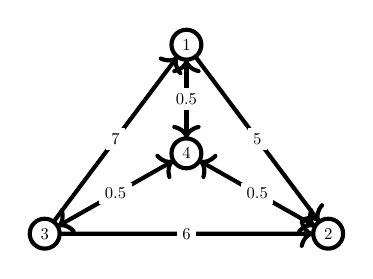
\begin{tikzpicture}
[scale=0.6, every node/.style={transform shape}]
    \SetVertexNormal[Shape      = circle,
    FillColor = white,
    LineWidth  = 1.5pt]
    \SetUpEdge[lw         = 1.5pt,
    color      = black,
    labelcolor = white]

    \tikzset{node distance = 1.6in}

    \tikzset{VertexStyle/.append  style={fill}}
    \Vertex[x=0,y=0]{1}
    \Vertex[x=3,y=-4]{2}
    \Vertex[x=-3,y=-4]{3}
    \Vertex[x=0,y=-2.3]{4}
    \tikzset{EdgeStyle/.style={->}}
    \Edge[label=5](1)(2)
    \Edge[label=6](3)(2)
    \Edge[label=7](3)(1)
    \tikzset{EdgeStyle/.style={<->}}
    \Edge[label=0.5](1)(4)
    \Edge[label=0.5](4)(3)
    \Edge[label=0.5](4)(2)
\end{tikzpicture}
\caption{A benefits matrix ${B}({0})$ and its graphical depiction, in which player \#4 is essential despite providing smaller benefits than the others.}
\label{fig:three-cycle-2}
\end{figure}


\paragraph{Spectral Radius in Terms of Cycles}


Gelfand's formula for the spectral radius helps us articulate the role cycles play in Pareto improvements.


\begin{fact}\label{fact:cycles}\label{fact:monotonic}
For any nonnegative matrix ${M}$, its spectral radius $\rho({M})$ is equal to $ \limsup_{t \to \infty} \trace \left({M}^t\right)^{1/t} .$


\end{fact}


For a directed, unweighted graph with adjacency matrix ${M}$, the quantity $\trace \left({M}^t\right)$  measures the strength of all closed walks of length $t$ by taking the product of the edge weights for each such walk, and then summing these values over all such walks.

The essential agents discussed in the last section will be those that are present in sufficiently many of the high value cycles in the network. Relatedly, a single weak link in a cycle will dramatically reduce the value of that cycle. Thus networks with an imbalanced structure, in which it is rare for those agents who could confer large marginal benefits on others to be the beneficiaries of others' efforts, will have a lower spectral radius and there will be less scope for cooperation.



\section*{Markets and Imperfect Measurement}

Practically-minded readers may have a nagging worry. Imagine one of the models we have presented actually describes an economic situation. How can an analyst use these models without direct access to the data we have taken as given (e.g., the matrices $M$ or $B$)? In practice, such objects are, at best, observed imperfectly. 

This section exposits an approach to this in the context of a network game from the theory of firm behavior from \cite{GaleottiGolubGoyalTalamasTamuz2024}, which also illustrates how network game theory can be applied to situations with traditional economic ingredients, such as prices and quantities. The agents in this model are \( n \) firms (businesses), selling distinct goods  (e.g., computers, VR headsets, math textbooks, etc.).  Each chooses an action $x_i$, which is the price of its good. Quantities sold as a function of prices are $q(x)=q^0+Mx$, where $q^0 \in \mathbb{R}^n$ and $M$ is an $n$-by-$n$ matrix satisfying the normalization $M_{ii}=-1$ for all $i$. A firm pays a cost $c_i$ per unit sold, and firm $i$'s profits are $ u_i(x) = q_i(x)(p_i-c_i).$ Solving for the Nash equilibrium of the game yields the following analogue of \cref{eq:Nash}: when costs are perturbed by $\dot{c}$, equilibrium prices are perturbed by $$ \dot{x} = (I-M)^{-1} \dot{c}.$$ 

An economically important feature of this model is that \emph{market outcomes are Pareto inefficient}: markets in this model can have their outcomes improved, from a social perspective, by thoughtful interventions.\footnote{The basic idea is that when firms set prices, they do not have an incentive to focus on economic surplus that is not part of their profit. As a result, they can set ``socially inefficient'' prices, typically higher than a welfare-minded planner would. Interventions by authorities such as platform operators (e.g., Amazon) or government agencies can remedy this, at least partially.} We thus introduce an authority that can influence the game by choosing an \emph{intervention}, a vector \( \sigma \in \mathbb{R}^n \) which perturbs firms' costs, $\dot{c}=-\sigma$.  The effect of the intervention on \emph{economic surplus} (a measure of welfare inclusive of effects on firms, consumers, and the authority's expenditure) turns out to be
\begin{equation}
V(\sigma) = (q^0)^\top (I - M)^{-1} M \sigma, \label{eq:welfare_market}
\end{equation} where $q^0 \in \mathbb{R}^n$ is a given vector of pre-intervention quantities. This follows by some standard calculations spelled out in \cite{GaleottiGolubGoyalTalamasTamuz2024}, and we will take this more elaborate version of \cref{eq:welfare_game} for granted.




We now formulate the authority's problem, which, in essence, is to improve economic surplus with high confidence despite very noisy information. We posit that the authority observes noisy estimates of \( M \) and $q^0$, denoted by $$ \widehat{M} = M + E \quad \text{ and } \quad  \widehat{q}^0 = q^0 + z,$$ where \( E \) and $z$ are a random matrix and a random vector modeling estimation error. Practically, econometricians (economic statisticians) have developed tools to estimate market quantities $q^0$ and effects of each firm's pricing on other firms' demands ($M$). We will assume that $E$ is symmetric, and its upper-triangular entries are independent and identically distributed with a variance uniformly bounded in $n$; we will assume the same of the entries of $z$. The challenge  for the authority is that any intervention causes ripple effects through strategic behavior, captured by the matrix $(I-M)^{-1}$ in \cref{eq:welfare_market}. Readers familiar with numerical analysis will recognize that $(I-M)^{-1}$ can be extremely sensitive to mismeasurement. In other words, an authority that does not know these ripple effects exactly might worry about doing harm with an intervention. To formalize this, we will consider a planner who knows that $(M,q^0)$ lies in some known set of possibilities $\mathfrak{P}$ and seeks a robust intervention rule:
\begin{problem} An $\epsilon$-\emph{robust intervention rule} for $\mathfrak{P}$ is a function $\sigma(\widehat{M})$ so that, for all $(M,q^0) \in \mathfrak{P}$ we have $V(\sigma(\widehat{M})) \geq 1$ with probability at least $1-\epsilon$. \end{problem}

Note the randomness is only in the draw of $E$. 

We will give conditions under which robust interventions exist. Define the subspace \( \mathcal{L}(M, \mu) \subseteq \mathbb{R}^n \) as the span of eigenvectors of \( M \) corresponding to eigenvalues \( \lambda \) with \( |\lambda| \geq \mu \).
\begin{definition} The pair $(M,q^0)$ has \( (\mu, \delta) \)-\emph{recoverable structure} if the projection of \( q^0 \) onto \( \mathcal{L}(M, \mu) \)  has norm at least $\delta$.\end{definition} Note this condition requires that $M$ has some eigenvalues larger than $\mu$, and that $q^0$ projects nonvanishingly onto those eigenspaces.
Then we have:
\begin{prop}
  Fix $\delta>0$ and a sequence $\mu(n) \in \omega(\sqrt{n})$. If all pairs in $\mathfrak{P}$ have  \( (\mu(n), \delta) \)-recoverable structure, then $\epsilon$-robust intervention rules exist for some $\epsilon>0$ and all large enough $n$.  
\end{prop}

The significance of the condition $\mu(n)/\sqrt{n} \to \infty$ is that the Frobenius norm of $E$ is $O(\sqrt{n})$ by the theory of Wigner matrices. In this sense, the condition says that all possible markets in $\mathfrak{P}$ have recoverable structure ``larger'' than the norm of the noise. We now sketch how this is used to intervene robustly.

Let's diagonalize the matrix \( M \):
\[
M = W \Lambda W^\top,
\]
where \( W \) is orthogonal with columns $u_\ell$ and \( \Lambda \) is diagonal with entries \( \lambda_\ell \). We can write the effect on welfare of an intervention as \begin{equation} \label{eq:V_market_spectral}
V(\sigma) = \sum_{\ell=1}^n \alpha_\ell \beta_\ell \frac{\lambda_\ell}{1 - \lambda_\ell},
\end{equation}
where \( \sigma = \sum_{\ell=1}^n \alpha_\ell w^\ell \) and  \( q^0 = \sum_{\ell=1}^n \beta_\ell w^\ell \), where $w^\ell$ are the columns of $W$. 

The challenge in making this quantity positive with an intervention is that the authority does not know the true $M$ or its eigenvectors $U$; it only has access to the noisy proxy $\widehat{M}$. 

Nevertheless, the spectral rewriting of the welfare function is useful, because it allows us to use the Davis--Kahan theorem, which can guarantee precise recovery of some of the spectral summands. Let $\widehat{U}$ be the matrix of eigenvectors that diagonalizes $\widehat{M}$. Let us first impose the additional technical condition that the largest eigenvalue $\lambda_1$ is separated from the second-largest by a sufficiently large gap---much larger than $\sqrt{n}$.  In that case, the Davis--Kahan theorem guarantees that the eigenvector $\widehat{u}_1$ is very close to $u_1$. This opens the door for the authority to effectively control the first summand of \cref{eq:V_market_spectral}, while keeping all the other summands nearly zero. That is the essence of the ``robust intervention'' strategy. 




Intuitively, the noise in $\widehat{M}$ means that many specific spillovers cannot be known precisely. But the identification of some large-eigenvalue eigenspaces permits the detection and estimation of latent patterns in the interactions that have a strong impact on demand responses $q(x)=q^0+Mx$. This turns out to be enough for designing good interventions.

For the strategy we have sketched to work in general, several important details have to be dealt with. First, the ``gap'' condition separating the largest eigenvalue from the rest might not hold. In this case, the authority may be forced to approximate a space $\mathcal{L}(M, \mu)$ of dimension exceeding $1$, which makes the tailoring of \cref{eq:V_market_spectral} to be positive more delicate. Second, some assumptions are needed to make sure that $\beta_\ell$ are not all too small; if they are, then statistical noise can make the tailoring impossible. The assumption on $q^0$ in the definition of recoverable structure is related to this issue.

\paragraph{Illustration} To illustrate our approach, consider a matrix $M=M_{\text{block}}$ for $n=300$ 
where $M_{\text{block}} = C \otimes J_{n/3}$, where
\[ C = \begin{pmatrix} -1 & 0.15 & 0.7 \\ 0.15 & -1 & 0.6 \\ 0.7 & 0.6 & -1 \end{pmatrix} \]
and $J$ is the matrix of ones. The top eigenvalue of $M$ is about $200$, while if $E$ has standard normal entries, its largest eigenvalue is about $30$. This allows the top eigenvector $u^1$ of $M$ to be recovered from $\widehat{M}$, as illustrated in   \Cref{fig:sampling_figure}.



\section*{Closing Reflections} 

The previous section illustrates a large practical payoff of reformulating economic problems in spectral terms: we can use statistical results on the recovery of eigenvalues and eigenvectors through noisy observation and sampling. Such recovery strategies constitute a rich and active area of research. Connections to economics promise new applications as well as new mathematical questions \cite{chen2021spectral}.

We have focused on the setting of market games to illustrate this interplay simply because that is where the existing research on the topic is. But exploiting the synergy between ``spectral microeconomics'' and statistics offers exciting avenues in all the applications we have mentioned. One that I would like to emphasize is the public goods model. It is, in my view, urgent to improve mechanisms for providing public goods in areas ranging from climate change to the management of new artificial intelligence technologies. Economic mechanisms that deal not only with incentive issues but also with the statistical uncertainties inherent in measuring spillovers are urgently needed. The ideas we have presented may be useful tools for building such mechanisms.


 





\bibliography{refs}


\newpage 
\onecolumn




\begin{figure}[ht!]
    \centering
    \begin{subfigure}[b]{0.45\textwidth}
        \centering
        \adjincludegraphics[width=\textwidth,trim={1cm 7cm 2cm 8.49cm},clip]{graphs/gamma=0,_sampling=1/D_true.pdf}
        \caption{True  matrix $M$}
        \label{fig:sub1_matrix}
    \end{subfigure}
    \hfill
    \begin{subfigure}[b]{0.45\textwidth}
        \centering
        \adjincludegraphics[width=\textwidth,trim={1cm 7cm 2cm 8.49cm},clip]{graphs/gamma=0,_sampling=1/Rank1_D_true.pdf}
        \caption{True first spectral summand: ${w}^1 ({w}^1)^\tr$}
        \label{fig:sub2_matrix}
    \end{subfigure}
    \vskip 0.5\baselineskip
    \begin{subfigure}[b]{0.45\textwidth}
        \centering
        \adjincludegraphics[width=\textwidth,trim={1cm 7cm 2cm 8.49cm},clip]{graphs/gamma=0,_sampling=1/D_observed.pdf}
        \caption{Noisy observation $\widehat{M}$}
        \label{fig:sub3_matrix}
    \end{subfigure}
    \hfill
    \begin{subfigure}[b]{0.45\textwidth}
        \centering
        \adjincludegraphics[width=\textwidth,trim={1cm 7cm 2cm 8.49cm},clip]{graphs/gamma=0,_sampling=1/Rank1_D_observed.pdf}
        \caption{Estimated first spectral summand: $\widehat{{w}}^1 (\widehat{{w}}^1)^\tr$}
        \label{fig:sub4_matrix}
    \end{subfigure}
    \caption{Illustration of true vs. estimated parameters in the example. Blue pixels correspond to negative matrix entries, while the red regions to positive ones. The spectral summand refers to the first term in the spectral decomposition $M=\sum_{\ell=1}^n \lambda_\ell w^\ell (w^\ell)^\tr$.}
  \label{fig:sampling_figure}
\end{figure}




\end{document}
